\documentclass[modern]{rnaastex}

\pdfoutput=1

\usepackage{microtype}
\usepackage{url}
\usepackage{amsmath}
\usepackage{amssymb}
\usepackage{natbib}
\usepackage{multirow}
\bibliographystyle{aasjournal}

% ------------------ %
% end of AASTeX mods %
% ------------------ %

% Projects:
\newcommand{\project}[1]{\textsf{#1}}
\newcommand{\kepler}{\project{Kepler}}

% references to text content
\newcommand{\documentname}{\textsl{Note}}
\newcommand{\figureref}[1]{\ref{fig:#1}}
\newcommand{\Figure}[1]{Figure~\figureref{#1}}
\newcommand{\figurelabel}[1]{\label{fig:#1}}
\renewcommand{\eqref}[1]{\ref{eq:#1}}
\newcommand{\Eq}[1]{Equation~(\eqref{#1})}
\newcommand{\eq}[1]{\Eq{#1}}
\newcommand{\eqalt}[1]{Equation~\eqref{#1}}
\newcommand{\eqlabel}[1]{\label{eq:#1}}

% TODOs
\newcommand{\todo}[3]{{\color{#2}\emph{#1}: #3}}
\newcommand{\dfmtodo}[1]{\todo{DFM}{red}{#1}}
\newcommand{\alltodo}[1]{\todo{TEAM}{red}{#1}}
\newcommand{\citeme}{{\color{red}(citation needed)}}

% math
\newcommand{\T}{\ensuremath{\mathrm{T}}}
\newcommand{\dd}{\ensuremath{ \mathrm{d}}}
\newcommand{\unit}[1]{{\ensuremath{ \mathrm{#1}}}}
\newcommand{\bvec}[1]{{\ensuremath{\boldsymbol{#1}}}}
\newcommand{\Gaussian}[3]{\ensuremath{\frac{1}{|2\pi #2|^\frac{1}{2}}
            \exp\left[ -\frac{1}{2}#1^\top #2^{-1} #1 \right]}}

% VECTORS AND MATRICES USED IN THIS PAPER
\newcommand{\Normal}{\ensuremath{\mathcal{N}}}
\newcommand{\mA}{\ensuremath{\bvec{A}}}
\newcommand{\mC}{\ensuremath{\bvec{C}}}
\newcommand{\mS}{\ensuremath{\bvec{\Sigma}}}
\newcommand{\mL}{\ensuremath{\bvec{\Lambda}}}
\newcommand{\vw}{\ensuremath{\bvec{w}}}
\newcommand{\vy}{\ensuremath{\bvec{y}}}
\newcommand{\vt}{\ensuremath{\bvec{\theta}}}
\newcommand{\vm}{\ensuremath{\bvec{\mu}(\bvec{\theta})}}
\newcommand{\vre}{\ensuremath{\bvec{r}}}
\newcommand{\vh}{\ensuremath{\bvec{h}}}
\newcommand{\vk}{\ensuremath{\bvec{k}}}

% typography obsessions
\setlength{\parindent}{3.0ex}

\begin{document}\raggedbottom\sloppy\sloppypar\frenchspacing

\title{%
    Linear models for systematics and nuisances
}

\author[0000-0002-0296-3826]{Rodrigo Luger}
\affil{Department~of~Astronomy, University~of~Washington, Box 351580, Seattle, WA 98195, USA}

\author[0000-0002-9328-5652]{Daniel Foreman-Mackey}
\affil{Center for Computational Astrophysics, Flatiron Institute, 162 Fifth Ave, New York, NY 10010, USA}

\author[0000-0003-2866-9403]{David W. Hogg}
\affil{Center for Computational Astrophysics, Flatiron Institute, 162 Fifth Ave, New York, NY 10010, USA}
\affil{Center for Cosmology and Particle Physics, Department of Physics, New York University, 726 Broadway, New York, NY 10003, USA}
\affil{Center for Data Science, New York University, 60 Fifth Ave, New York, NY 10011, USA}
\affil{Max-Planck-Institut f\"ur Astronomie, K\"onigstuhl 17, D-69117 Heidelberg}

\keywords{%
methods: data analysis ---
methods: statistical
}

\section{Introduction}

The target of many astronomical studies is the recovery of tiny astrophysical
signals living in a sea of uninteresting (but usually dominant) noise.
In many contexts (for example, stellar time-series, or
high-contrast imaging, or stellar spectroscopy), there are structured
components to this noise caused by systematic
effects in the astronomical source, the atmosphere, the telescope, or
the detector.
More often than not, evaluation of the true physical model for these nuisances
is computationally intractable and dependent on too many (unknown) parameters
to allow rigorous probabilistic inference.

Sometimes housekeeping data, and often the science data themselves,
can be used as predictors of the systematic noise.
Linear combinations of these predictors (or linear combinations of non-linear functions
of these predictors) are often used as
computationally tractable models that can capture the nuisances.
These linear models---that is, linear combinations of (possibly nonlinear) functions
of various systematic predictors---can be used to fit and subtract systematics prior to
investigation of the signals of interest, or they can be used in a
simultaneous fit of the systematics and the signals.
For our purposes, a \emph{linear model} for a column vector of data $\vy$
can be written in the form
\begin{align}
\eqlabel{linearmodel}
\bvec{y} = \vm + \mA \vw + \mathrm{noise}
\end{align}
where $\vm$ is the column-vector expectation or mean model or the part of the model
that we care about, $\mA$ is a \emph{design matrix}, whose columns are basis
vectors $\{\bvec{a}_j\}$ or predictors for the systematics,
and $\vw$ is the vector of weights or amplitudes, one
for each basis vector.

Similar models have been used to describe the systematics in astrophysical time
series data \citep{Smith:2012, Wang:2016, Luger:2016}, galaxy or stellar spectra
\citep{Tsalmantza:2012, Ness:2015}, and imaging \citep{Fergus:2014,
Wang:2017}.
One issue with flexible data-driven models, however, is their tendency to
over-fit and reduce the astrophysical signal of interest.
This is generally tackled using a dimensionality reduction technique like
principal component analysis (PCA) or by applying strong priors or a
regularization to the weights vector $\vw$.

In this \documentname, we show that if a
Gaussian prior is placed on the weights $\vw$ of the linear
components, the weights can be marginalized out with an operation in pure linear
algebra, which can (often) be made fast.
We illustrate this model by demonstrating the applicability of a linear model
for the non-linear systematics in \kepler\ time-series data, where the dominant
noise source for many stars is spacecraft motion and variability.

\section{The problem}

Consider a dataset $\vy$ of $N$ measurements $y_i$ with covariance
matrix $\mC$.
In the common case of data collected with measurement error $\sigma_i$ on
individual data points but no correlation across measurements, $\mC$ is a
diagonal matrix with $\mC_{ij} = \sigma_{i}\delta_{ij}$, although in general
the off-diagonal elements capture the covariance between different
measurements. Given a mean function $\vm$  and a linear model as in
\eq{linearmodel}, the probability of the data under the model is given by a
normal distribution with mean $\vm + \mA \vw$ and variance $\mC$:
%
\begin{align}\eqlabel{likelihood}
p(\vy | \vt, \vw) &= \Normal(\vy; \vm + \mA \vw, \mC) \quad.
\end{align}
%
However, we are specifically not interested in the \emph{value} of $\vw$.
Instead, we will marginalize over it.
To perform this marginalization we must place a prior on $\vw$ that we will
assume to be Gaussian
%
\begin{align}
p(\vw) &= \Normal(\vw; 0, \mL) \quad. \nonumber
\end{align}
%
With this prior and likelihood in \eq{likelihood}, our goal is to marginalize
out the weights $\vw$; that is, we want to compute the marginalized
likelihood
%
\begin{align}
p(\vy | \vt) &= \int_{-\infty}^{\infty} p(\vw)\,p(\vy | \vt, \vw) \dd\vw
\end{align}
and we would like to do it without doing any numerical integrals, and without
explicitly solving for the weights $\vw$.

\section{The solution}

The marginalized likelihood may be expressed as follows (see Appendix):
%
\begin{align}
\eqlabel{p(y|t)normal}
p(\vy | \vt) &= \Normal (\vy; \vm, \mC + \mA \mL \mA^\top) \quad.
\end{align}
%
This marginalized likelihood function can be numerically maximized to find the
maximum likelihood parameters $\theta^\star$ or this likelihood can be
multiplied by a prior $p(\theta)$ and used for posterior inference.
In either case, the evaluation of the model will include the effects of
marginalizing over $\bvec{w}$ in the linear model and any uncertainties in
those values will be propagated to the results.

It is often useful to compute the value of the linear model so that we can
``remove'' systematics from the data.
To derive this, we recognize that \eq{p(y|t)normal} is the likelihood of a
Gaussian Process.
This means that conditioned on the data and a choice of the parameters
$\bvec{\theta}$, the systematics will have a Gaussian distribution with mean
$\bvec{m}$ and covariance $\bvec{\Sigma}_\bvec{m}$ given by
\citep{Rasmussen:2006}
%
\begin{align}\eqlabel{pred}
\bvec{m} &= \mu(\bvec{\theta}) + \mA \mL \mA^\top  \left[\mC +
    \mA \mL \mA^\top\right]^{-1} \left[\bvec{y} - \mu(\bvec{\theta})\right]
    \nonumber\\
\bvec{\Sigma}_\bvec{m} &= \mA \mL \mA^\top - \mA \mL \mA^\top
    \left[\mC + \mA \mL \mA^\top\right]^{-1}
    \mA^\top \mL \mA \quad.
\end{align}

\begin{figure}[h!]
\begin{center}
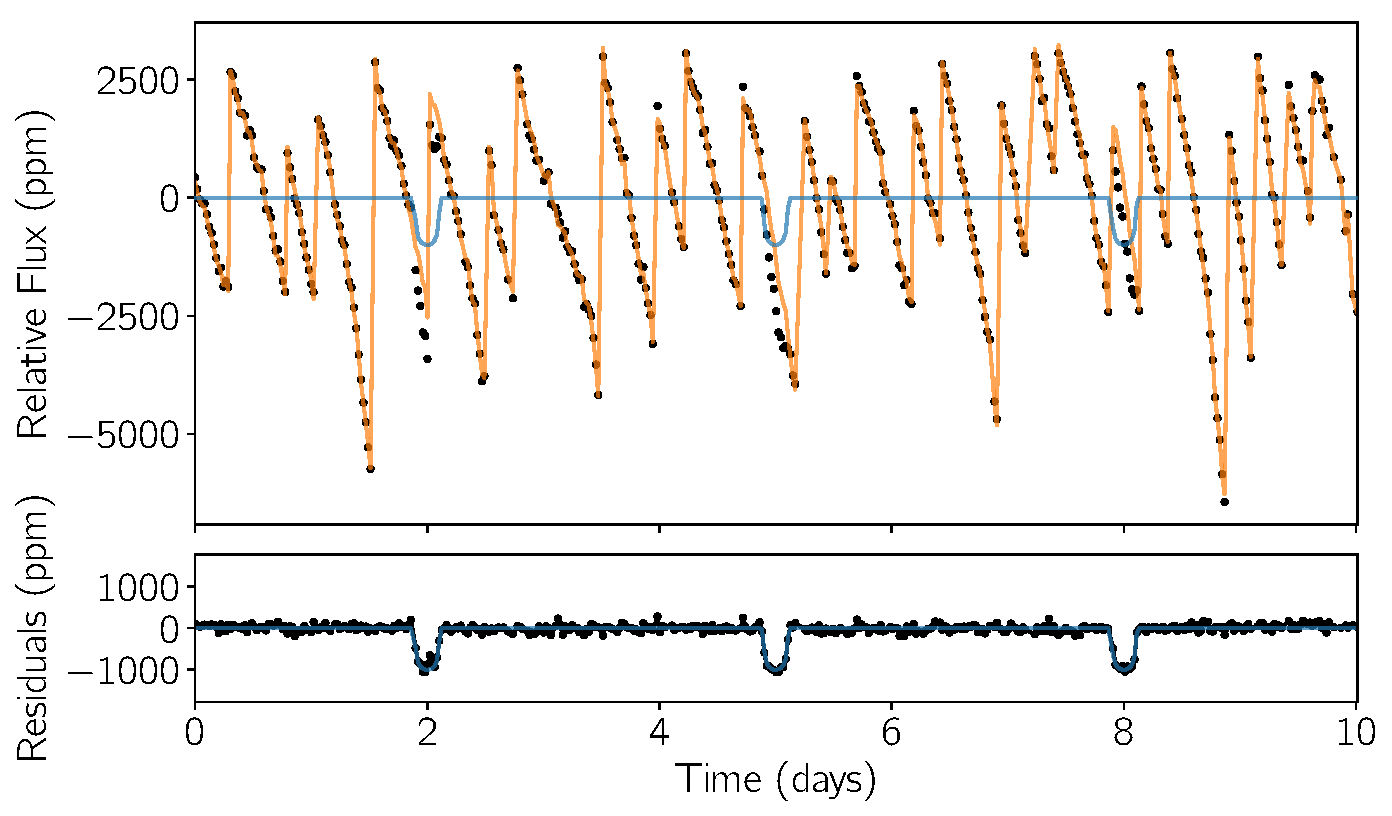
\includegraphics[width=0.9\textwidth]{figure.pdf}
\caption{%
(top): The black points show the raw light curve for the \project{K2} target
    EPIC~204832142 multiplied by the time series for a simulated transiting
    planet.
    The simulated transit model is shown as a blue line.
    We fit the systematics using the linear model from the \project{everest}
    library \citep{Luger:2016, Luger:2017} and the prediction for the
    systematics model (\eqalt{pred}) are shown as an orange line.
(bottom): The same data from the top panel with the systematics model
    subtracted.
    The transit model is plotted in blue.
\figurelabel{figure}}
\end{center}
\end{figure}

\section{The implications}

\alltodo{What new powers has this given us and how will we use them for good?}

\acknowledgements
It is a pleasure to thank
  Patrick Cooper (Duquesne),
  Boris Leistedt (NYU),
  Bernhard Sch\"olkopf (MPI-IS), and
  Dun Wang (NYU)
for helping us understand all of this.

\bibliography{linear}

\section{Appendix}

The marginalized likelihood may be expressed as follows:
\begin{align}
\eqlabel{integral}
p(\vy | \vt) &= \frac{1}{|2\pi\mL|^\frac{1}{2} |2\pi\mC|^\frac{1}{2}}
                \int_{-\infty}^{\infty} \exp \left[ -\frac{1}{2} z \right] \dd\vw
\end{align}
%
where
%
\begin{align}
\eqlabel{z}
z &= \vw^\top \mL^{-1} \vw + (\vre - \mA \vw)^\top \mC^{-1} (\vre - \mA \vw)
\end{align}
%
and $\vre = \vy - \vm$.
%
The integral in \eq{integral} is easier to evaluate if we
complete the square and write:
%
\begin{align}
\eqlabel{z_square}
z &= (\vw - \vh)^\top \mS^{-1} (\vw - \vh) + k \quad,
\end{align}
%
where, by comparison with \eq{z}, it can be shown that
%
\begin{align}
\mS^{-1} &= \mL^{-1} + \mA^\top \mC^{-1} \mA \\
%
\vh &= \bvec{\Sigma} \mA^\top \mC^{-1} \vre \\
%
k &= \vre^\top \left( \mC^{-1} - \mC^{-1} \mA \mS \mA^\top \mC^{-1} \right) \vre
    \quad.
\end{align}
%
We may thus write
%
\begin{align}
\eqlabel{p(y|t)ugly}
p(\vy | \vt) &= \frac{1}{
                |2\pi\mL|^\frac{1}{2}
                |2\pi\mC|^\frac{1}{2}}
                \exp \left[ -\frac{1}{2}k \right]
                \int_{-\infty}^{\infty} \exp
                \left[-\frac{1}{2}(\vw - \vh)^\top \mS^{-1} (\vw - \vh)
                \right] \dd\vw \quad.
\end{align}
%
The integral is that of a Gaussian, which evaluates to
$|2\pi\bvec{\Sigma}|^\frac{1}{2}$.
By the Matrix Determinant Lemma and the Woodbury Identity
\citep[for example,][]{Woodbury:1950, Harville:1997},
%
\begin{align}
|\mS| &= {|\mS^{-1}|}^{-1} = \frac{|\mL| |\mC|}{|\mC + \mA \mL \mA^\top|} \nonumber \\
k &= \vre^\top \left( \mC + \mA \mL \mA^\top \right)^{-1} \vre \quad.
\end{align}
%
Combining these results, the expression in \eq{p(y|t)ugly} simplifies to
\begin{align}
\eqlabel{p(y|t)exp}
p(\vy | \vt) &= \frac{1}{
                |2\pi(\mC + \mA \mL \mA^\top)|^\frac{1}{2}}
                \exp \left[ -\frac{1}{2} \big( \vy - \vm \big)^\top
                            (\mC + \mA \mL \mA^\top)^{-1}
                            \big( \vy - \vm \big)
                     \right] \quad.
\end{align}
%
This is a normal distribution with mean $\vm$ and covariance
$\mC + \mA \mL \mA^\top$:
%
\begin{align}
\eqlabel{p(y|t)normal}
p(\vy | \vt) &= \Normal (\vy; \vm, \mC + \mA \mL \mA^\top) \quad.
\end{align}

\end{document}
